La sesi\'on analizada cuenta con un total de 70 senadores,
pertenecientes a 27 partidos pol\'iticos, distribuidos del
siguiente modo (figura \ref{fig-distrib-senators}): 
solo uno de los partidos (Frente de todos) cuenta con 12
senadores; tambi\'en uno solo (Alianza frente para la victoria) es
representado por 10 senadores; dos partidos (Alianza cambiemos y
Juntos por el cambio) cuentan con 7 senadores, y el resto de los
partidos tienen entre 3, 2 y un senador.
En cuanto a las provincias (24 en total), todas tienen 3 senadores
exceptuando a Tucum\'an y a La Rioja que tienen solo 2.

De los votos emitidos, se observa que 38 son positivos; 29, negativos;
2 son ausencias, y uno es una abstenci\'on.
Como muestra la figura \ref{fig-distrib-vote}, la intenci\'on
de voto no guarda una relaci\'on un\'ivoca con los partidos a los cuales los
senadores representan. A excepci\'on de aquellos que cuentan con un \'unico
senador, la mayor\'ia es representado por senadores que votaron a favor y senadores
que votaron en contra de la ley para el acceso al aborto.

\begin{figure}[h!]
    \centering
    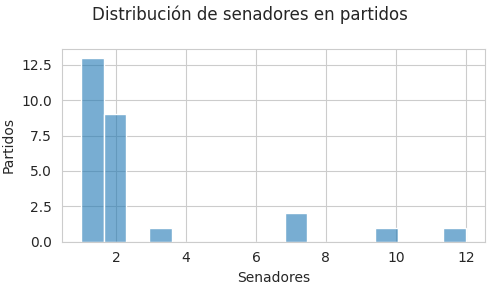
\includegraphics[scale=0.7]{./images/graphs/distrib_histplot_senators_parties.png}
    \caption{Distribuci\'on de senadores en partidos pol\'iticos.}
    \label{fig-distrib-senators}
\end{figure}

\begin{figure}[h!]
\centering
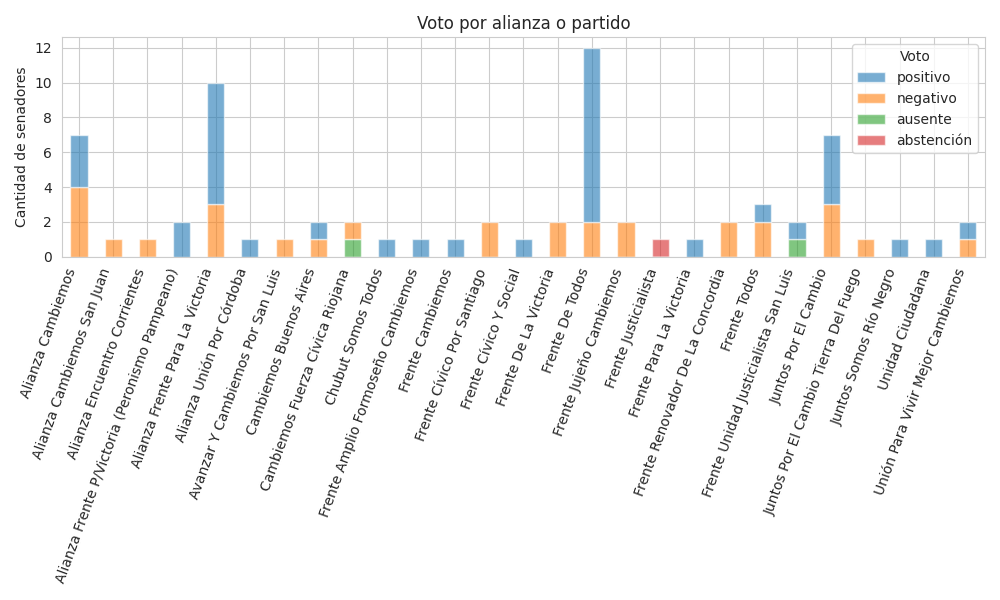
\includegraphics[scale=0.48]{./images/graphs/senators_vote_by_party.png}
\caption{Distribuci\'on de votos en los distintos partidos pol\'iticos.}
\label{fig-distrib-vote}
\end{figure}

Respecto de las intervenciones discursivas, se encuentran 111 discursos
por parte de los senadores que votaron a favor de la ley; 88 discursos por parte
de quienes votaron en contra; un discurso de quienes estuvieron ausentes
durante la votaci\'on, y uno de quien se abstuvo de votar.
Si se ponen en relaci\'on estos datos absolutos con la cantidad de senadores,
se ve que, en promedio, se emitieron
2.87 discursos por senador, con un desv\'io est\'andar de 6.23 y una mediana de 1,
coincidente adem\'as
con la moda, lo que nos indicar\'ia que se trata de una distribuci\'on asim\'etrica a derecha.
Estas medidas de centralidad incluyen a 9 senadores que no intervinieron en
la sesi\'on.
Al desagregar los datos seg\'un elecci\'on en la votaci\'on, es posible notar que las
abstenciones no presentan
dispersi\'on y su media se ubica en el valor 1. Esto se debe a que solo un senador
se abstuvo de votar y, a su vez, solo emiti\'o un discurso.
Una situaci\'on similar se da en las ausencias, donde tambi\'en se observa un \'unico discurso.
Pero dado que dos senadores estuvieron ausentes, la media se ubica hacia el valor $0.5$ y
el desv\'io, hacia el $0.7$.
En cuanto a los votos negativos y positivos, ambos presentan una moda de 1,
pero los negativos
exhiben una media y un desv\'io est\'andar mayor que los positivos
($3.03\pm8.43$ \textit{versus} $2.92\pm4.26$, respectivamente).
La figura \ref{fig-distrib-speech} muestra las distribuciones detalladas.

\begin{figure}[h!]
    \centering
    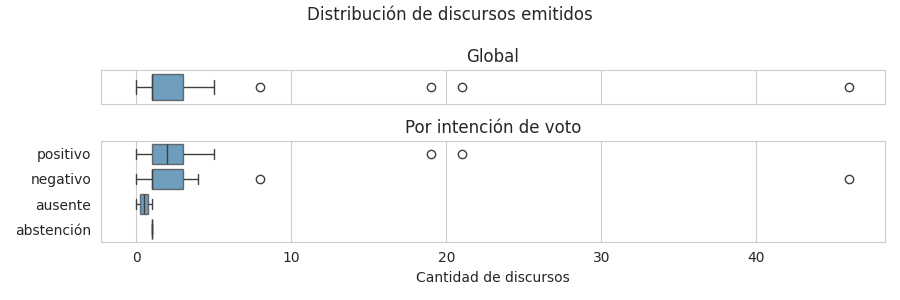
\includegraphics[scale=0.5]{./images/graphs/speech_by_vote.png}
    \caption{Distribuci\'on de votos en los distintos partidos pol\'iticos.}%
    \label{fig-distrib-speech}
\end{figure}

Como señalan \cite{bird2009natural}, las cadenas de caracteres ``incluyen muchos detalles
en los cuales no estamos interesados tales como espacios en blanco, saltos de l\'inea
y l\'ineas blancas [...] Para nuestro procesamiento del lenguaje, queremos dividir
estas cadenas en palabras y puntuaci\'on  [...] A este paso se lo llama
\textbf{tokenizaci\'on} y produce una estructura que nos es familiar.''
\footnote{Cita traducida del ingl\'es por la autora de este trabajo.
El resaltado es del original.}
Siguiendo esta t\'ecnica, se procesaron los discursos y se calcul\'o su
longitud considerando solamente las palabras que los consituyen.
Se observ\'o que la distribuci\'on de la longigud, medida de este modo, var\'ia
dependiendo de si se mide los documentos en \textit{tokens} totales o \'unicos.
En promedio, los discursos emitidos tienen 418 palabras, con un desv\'io
est\'andar de 714; la mediana es de 11 y la moda, de 7. Sin embargo, estas medidas
reflejan las palabras totales utilizadas en cada intervenci\'on, sin considerar si se repiten
o no: cada ocurrencia de una palabra cuenta, sin importar si ya fue pronunciada en el mismo
discurso. Es por eso que, a fines comparativos, se tomaron tambi\'en las medidas de centralidad
de los \textit{tokens} \'unicos, las cuales mostraron una media de 161 palabras por discurso
con un desv\'io de 245, una mediana de 11 y una moda de 2. La figura \ref{fig-distrib-tokens}
refleja este contraste. Como es posible notar, si bien en ambos casos los discursos
muestran valores at\'ipicos respecto de su longitud, cuando esta se mide en palabras
totales se observa una mayor cantidad con valores m\'as extremos que
al medirla en \textit{tokens} \'unicos. En este \'ultimo caso, un
$20\percentsign$ de los registros son valores at\'ipicos, de los cuales solo el
$17\percentsign$ constituyen casos extremos, mientras que, al considerar
el total de palabras, se observan un $22\percentsign$ y $32\percentsign$
respectivamente.\footnote{Para este an\'alisis se utiliz\'o el
test de Tukey, que toma el rango intercuartil o \textit{IQR} (\textit{Q3-Q1}, donde
\textit{Q1} refiere al primer cuartil y \textit{Q3}, al terceo) y considera
valores at\'ipicos leves a aquellos que se encuentran entre
$Q1 - (1.5 * IQR) < x < Q3 - (1.5 * IQR)$ y, como extremos a los que est\'an entre
$Q1 - (3 * IQR) < x < Q3 - (3 * IQR)$.}

\begin{figure}[h!]%
    \centering%
    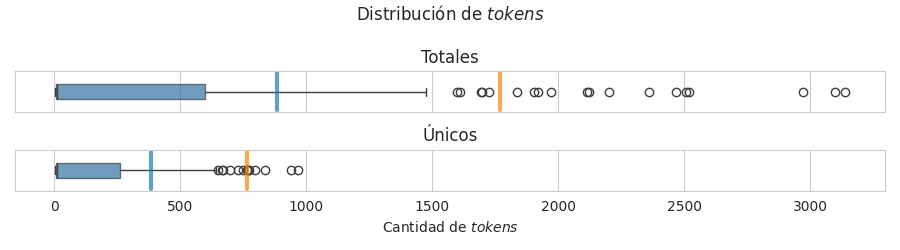
\includegraphics[scale=0.5]{./images/graphs/distrib_tokens.png}%
    \caption{Distribuci\'on de \textit{tokens} totales y \'unicos en los discursos pronunciados. En ambos gr\'aficos,
    la l\'inea azul indica el l\'imite a partir del cual una observaci\'on se considera at\'ipica leve
    ($IQR*1.5$) y la naranja, el l\'imite a partir del cual se la considera at\'ipica extrema ($IQR*3$).}%
    \label{fig-distrib-tokens}%
\end{figure}%
